\chapter{Our contributions}
\label{chap3}

\section{Triangulation adaptive to the local curvature}
\label{sub3.1}

As we explained in the begining of chapeter \ref{sub2.1}, curvature of the surface
is a measure of how much the surface bends.

The triangulation of the surface should be accurate enough, but also memory efficient.
This can be achieved by creating a triangulation which is locally adaptive to the
curvature of the surface. Therefore having smaller triangles in the places where
the surface is curved and having bigger triangles where surface is flatter.

In this section we present our implementation of the triangulation adaptive
to the local curvature.

In the original algorithm, the height of the triangle which is projected
to the surface is set to the constant value $\frac{\sqrt{3}}{2}e$, where $e$ 
is the required length of the side of the triangle. To achieve the adaptivity
of the triangles size, we set the height of the triangle to depend on the curvature in
the given point, as shown in the Figure \ref{img:15}.

\begin{figure}
    \centerline{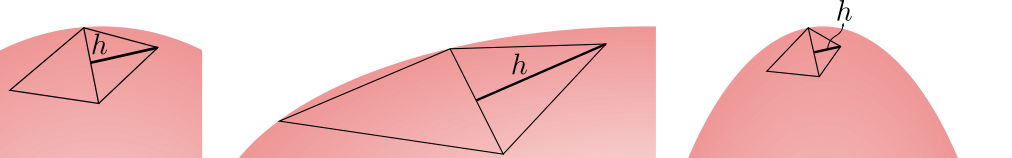
\includegraphics[scale=0.5]{images/img15}}
    \caption[Adaptive height of the new triangle]
    {Adaptive height of the new triangle.}
    %id obrazku, pomocou ktoreho sa budeme na obrazok odvolavat
    \label{img:15}
\end{figure}

To identify the curved areas, we decided to use the maximal curvature. As the minimal
and maximal curvature are both signed, we identify the areas depending on 
the absolute value of these curvatures.

We do not allow arbitrary height of the triangle to avoid edge-cases. We decided
to restrict the allowed height to $\frac{1}{4}\frac{\sqrt{3}}{2}e>h>4\frac{\sqrt{3}}{2}e$.
We create a variable $m-$multiplicator, depending on $\kappa_T$ and set the height of
the new triangle to $h=m\frac{\sqrt{3}}{2}e$.

As $\kappa_T$ has values in range $\langle 0, \infty \rangle$.

\begin{definition}
    Let us define triangulation curvature of the surface $S$ in the point $P=S(u, v)$ as
    $\kappa_T(u, v) = max(|\kappa_{min}|, |\kappa_{max}|).$
\end{definition}

NOT FINISHED YET

\section{Triangulation of ADE singularities}
\label{sub3.2}

\subsection{Analysis of the geometry of ADE singularities}

ADE singularities are simple, isolated surface singularities, which can be
expressed by corresponding implicit equations.

We already know, that $A_{1--}$ singularity is locally represented as a cone.
In this section we discuss geometric structure of other ADE surface singularities.

\begin{definition} (TODO rewrite)
    Let us define branch of ADE singularity as the part of the surface,
    which is connected to the rest only by the singular point.
\end{definition}

\begin{comment}
\begin{definition}
    Let us define triangulation direction of ADE singularity $A$ with radius $r$ as 
    Let us define triangulation direction of ADE singularity $A$ with radius $r$ as 
    a direction $\vec{v}$ for which 
    $$F\bigg(A+t \vec{v} \cap S_{r}(A)\bigg) < 0,$$
    where $F$ is the implicit equation defining the singularity $A$
    and $t,r \in \R^+$.
\end{definition}
As we can see, there are infinitely many axes of each ADE singularity.
\end{comment}

For our needs, we pick one triangulation vector for each branch of
each ADE singularity. This triangulation vector is normalized vector
either in the direction
of rotation symmetry axis or an intersection of reflection symmetry planes
of the corresponding branch. If the branch has only one reflection symmetry
plane, the triangulation vector is picked to lie in the reflection
symmetry plane.

\begin{comment}
Moreover, when placed to the singular point, triangulation vector of a branch 
is in the same half-space as the corresponding branch.
\end{comment}

In the general case, triangulation vectors serve us
as a partial information about the orientation of a singularity with 
respect to its normal form.

\subsubsection*{$A_n$ singularities}

As we can see from the equations 
$F(x,y,z)=x^{n+1}\pm y^2\pm z^2$, $A_{n-+}$
singularities are just rotated $A_{n+-}$ singularities and $A_{n++}$ singularities 
are a single point if $n$ is odd and reflected $A_{n--}$ singularities if $n$ is even. 
We therefore only discuss geometry of $A_{n--}$ and $A_{n+-}$ singularities.

$A_{n--}$ singularities are topologically equivalent to a cone if $n$ is odd, therefore
they have two branches.
If $n$ is even, they are topologically equivalent to a half cone or a plane, therefore
they have a single branch.
As $n$ gets bigger, the tip of the cone gets sharper. As $A_{n--}$ singularities
are rotationally symmetrical, we pick the direction of
axis of symmetry as triangulation vector. For a normal form, the triangulation vectors
are $(1, 0, 0)$ (and $(-1, 0, 0)$ if $n$ is odd).
First four $A_{n--}$ singularities can be seen on the Figure \ref{img:4}.

\begin{figure}
    \centerline{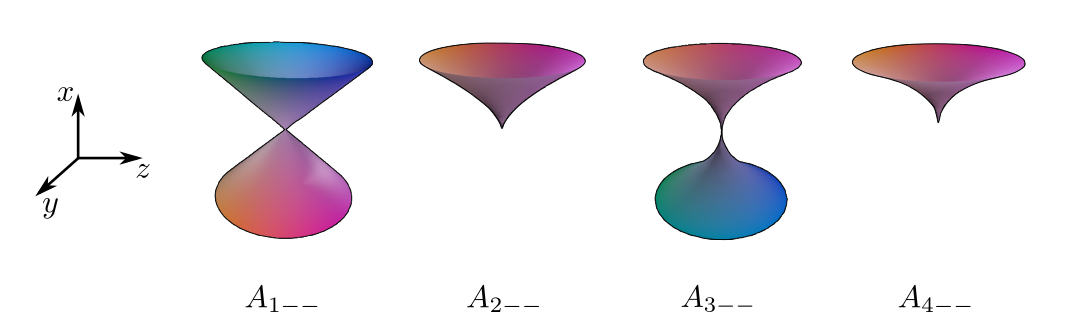
\includegraphics[scale=0.5]{images/img4}}
    \caption[$A_{n--}$ singularities]
    {$A_{n--}$ singularities. \cite{morris2003client}}
    %id obrazku, pomocou ktoreho sa budeme na obrazok odvolavat
    \label{img:4}
\end{figure}


$A_{n+-}$ singularities are topologically equivalent to a cone if $n$ is odd, therefore
they have two branches.
In the contrary with the previous singularities, as $n$ gets bigger, the tip
of the cone gets less sharp and flatter. Branches of these singularities have 
reflection symmetry planes $x=0$ and $y=0$, therefore we pick the vectors
$(0, 0, 1)$ and $(0, 0, -1)$ as the triangulation vectors.

If $n$ is even, $A_{n+-}$ singularities are topologically equivalent to a plane
with shape similar to hyperbolic paraboloid, therefore they have a single branch.
First four $A_{n+-}$ singularities can be seen on the Figure \ref{img:5}.
For this case, we pick the vector $(1, 0, 0)$ as a triangulation vector as
these singularities have reflection symmetry planes $y=0$ and $z=0$.

\begin{figure}
    \centerline{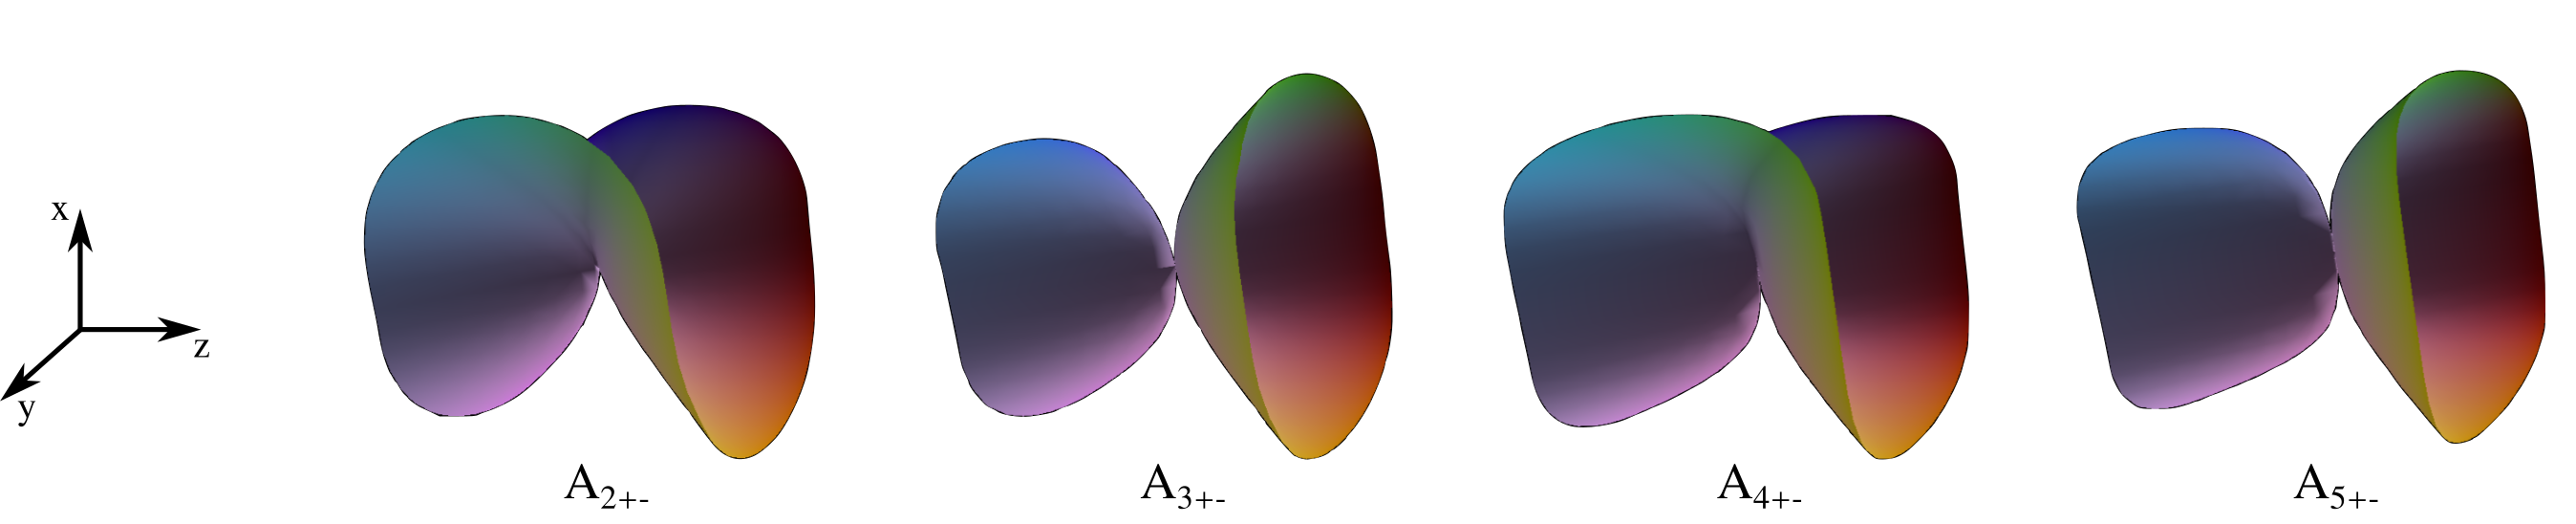
\includegraphics[scale=0.5]{images/img5}}
    \caption[$A_{n+-}$ singularities]
    {$A_{n+-}$ singularities. \cite{morris2003client}}
    %id obrazku, pomocou ktoreho sa budeme na obrazok odvolavat
    \label{img:5}
\end{figure}

\subsubsection*{$D_n$ singularities}

Given by equations $F(x,y,z)=yx^2\pm y^{n-1}\pm z^2$, we consider 8 categories.
For given sign combination and parity of n, the singularities are topologically
equivalent, with sharper(or flatter) features around the singularities for increasing
value of $n$ similar to $A_n$ singularities.

We can therefore say that $D_n$ singularities can be classified into 8 categories
locally represented by the following equations:
\begin{itemize}
    \item $D_{4++}$ \hspace{5mm} $yx^2 + y^3 + z^2$
    \item $D_{5++}$ \hspace{5mm} $yx^2 + y^4 + z^2$
    \item $D_{4+-}$ \hspace{5mm} $yx^2 + y^3 - z^2$
    \item $D_{5+-}$ \hspace{5mm} $yx^2 + y^4 - z^2$
    \item $D_{4-+}$ \hspace{5mm} $yx^2 - y^3 + z^2$
    \item $D_{5-+}$ \hspace{5mm} $yx^2 - y^4 + z^2$
    \item $D_{4--}$ \hspace{5mm} $yx^2 - y^3 - z^2$
    \item $D_{5--}$ \hspace{5mm} $yx^2 - y^4 - z^2$.
\end{itemize}

Now we look at some equivalences between these 8 categories.
$D_{4++}$ singularity is reflected $D_{4+-}$ singularity.
$D_{5++}$ singularity is reflected $D_{5--}$ singularity.
$D_{5-+}$ singularity is reflected $D_{5+-}$ singularity.
$D_{4-+}$ singularity is reflected $D_{4--}$ singularity.

We therefore only analyze geometry of $D_{n+-}$ singularities and
$D_{n--}$ singularities.

$D_{n+-}$ singularities are topologically equivalent to a plane when $n$ is
even and to a cone when $n$ is odd. Again, as $n$ gets bigger, the features
around singularities get sharper. Symmetry planes of these singularities
are $x=0$ and $z=0$, therefore we pick $(0, 1, 0)$ (and $(0, -1, 0)$ when $n$ is odd)
as triangulation vectors. First four $D_{n+-}$ singularities can be seen on
the Figure \ref{img:7}.

\begin{figure}
    \centerline{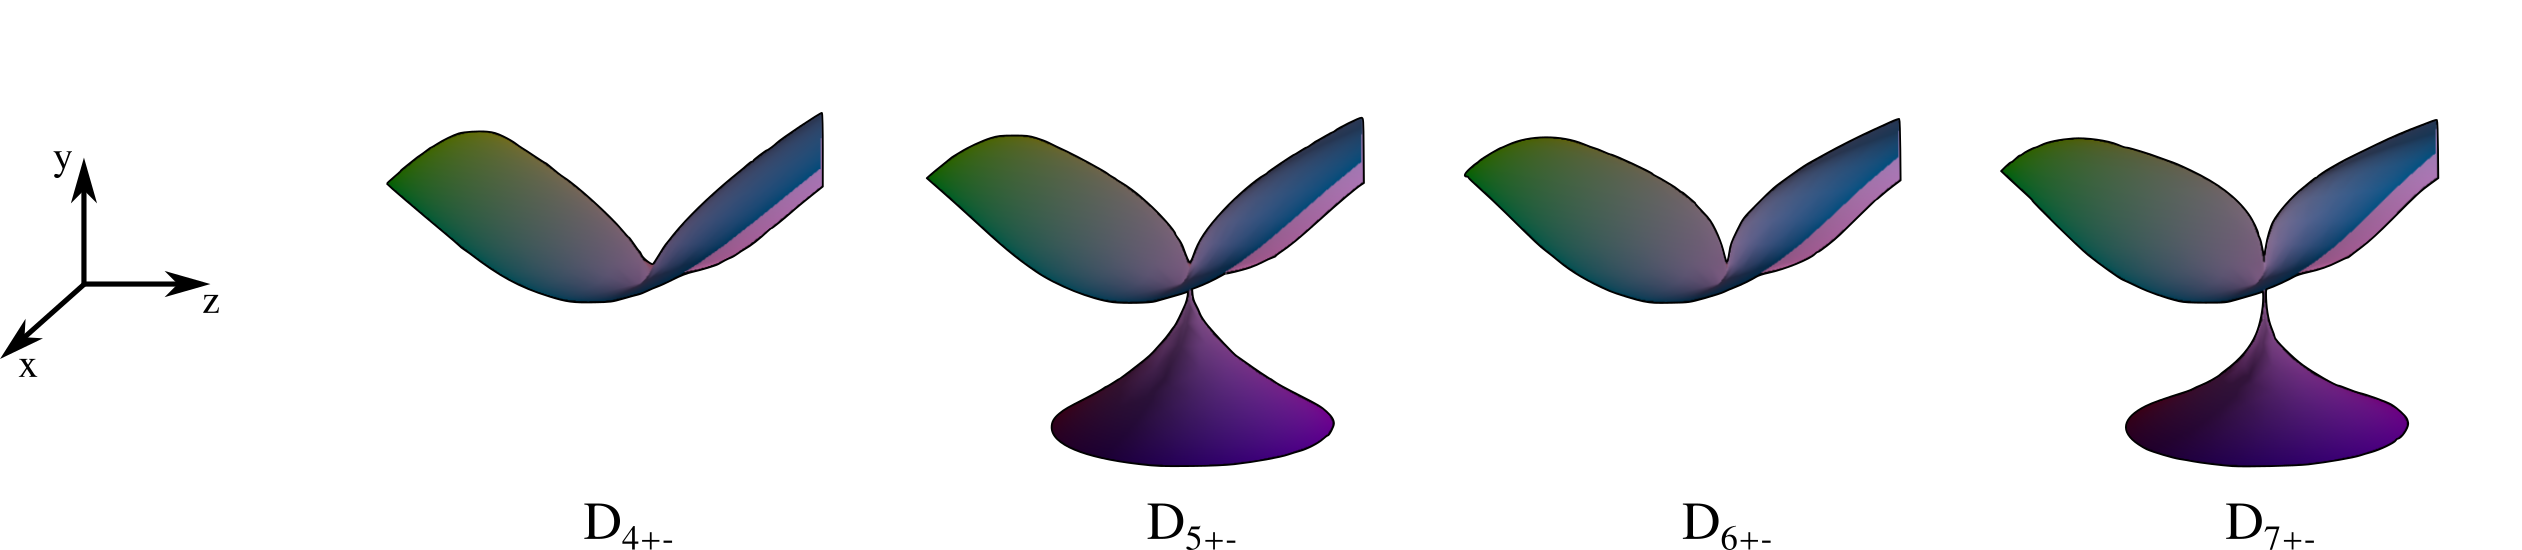
\includegraphics[scale=0.5]{images/img7}}
    \caption[$D_{n+-}$ singularities TODO the coordinates are wrong!!]
    {$D_{n+-}$ singularities. \cite{morris2003client}}
    %id obrazku, pomocou ktoreho sa budeme na obrazok odvolavat
    \label{img:7}
\end{figure}


$D_{n--}$ singularities are topologically equivalent to a cone when $n$ is
odd and to a 3 halfcones connected in the singular point when $n$ is even.
First four $D_{n--}$ singularities can be seen on the Figure \ref{img:8}.

\begin{figure}
    \centerline{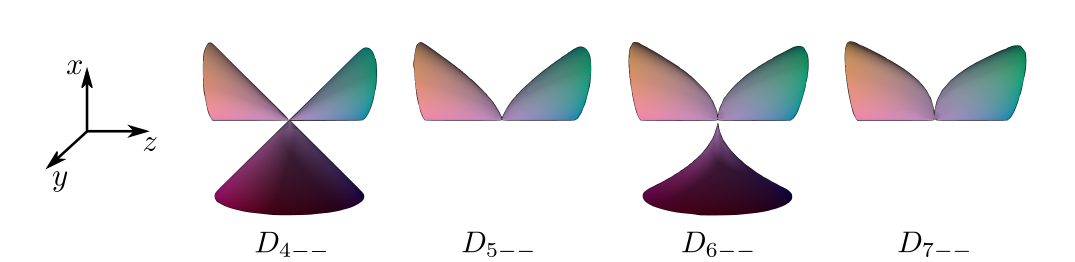
\includegraphics[scale=0.5]{images/img8}}
    \caption[$D_{n--}$ singularities TODO the coordinates are wrong!!]
    {$D_{n--}$ singularities. \cite{morris2003client}}
    %id obrazku, pomocou ktoreho sa budeme na obrazok odvolavat
    \label{img:8}
\end{figure}

Symmetry plane for all branches of these singularities is $z=0$.
the intersection of the surface and plane $z=0$ is displayed on the Figure \ref{img:6}.

\begin{figure}
    \centerline{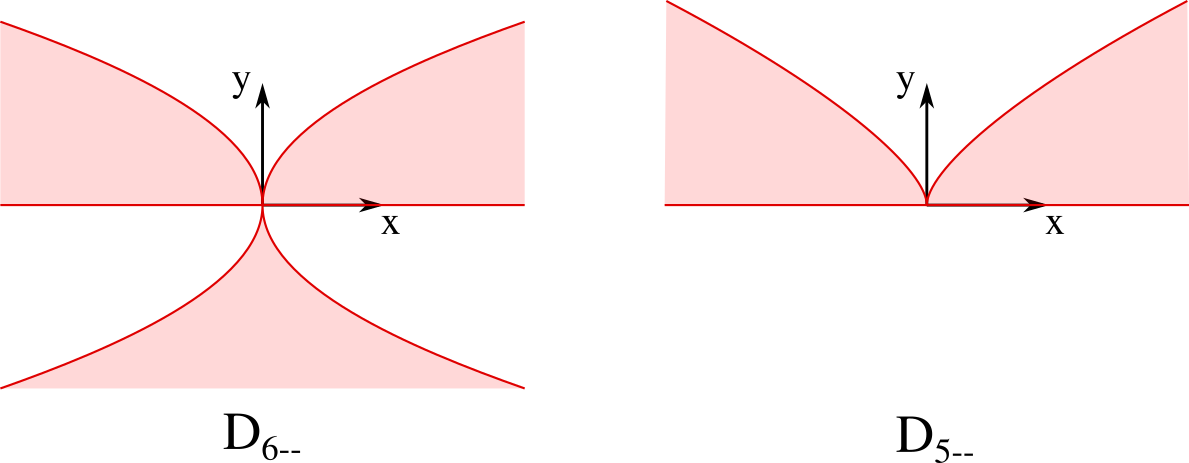
\includegraphics[scale=0.5]{images/img6}}
    \caption[Intersection of $D_{n--}$ singularities with plane $z=0$.]
    {Intersection of $D_{n--}$ singularities with plane $z=0$.}
    %id obrazku, pomocou ktoreho sa budeme na obrazok odvolavat
    \label{img:6}
\end{figure}

For $D_{n--}$ singularity, the intersections of the two branches where
$y \geq 0$ are bounded by curves $y=0$ and $x^2=y^{n-2}$. For given $r$,
we pick the triangulation vectors as $(r, \frac{1}{2}r^{\frac{2}{n-2}}, 0)$
and $(-r, \frac{1}{2}r^{\frac{2}{n-2}}, 0)$. The resulting vectors are
displayed on the Figure \ref{img:9} by blue arrow. Parameter $r$ is changed based
on the length of the edge of triangulation triangle.
displayed on the Figure \ref{img:9} by blue arrow. Parameter $r$ is changed based
on the length of the edge of triangulation triangle.

\begin{figure}
    \centerline{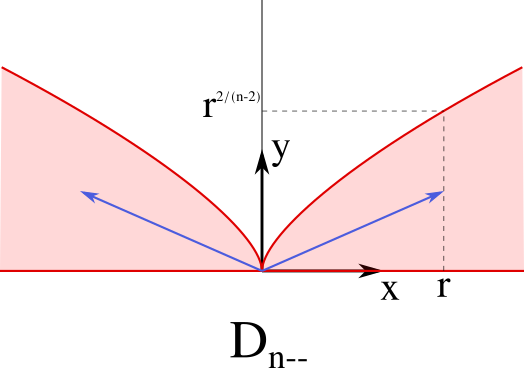
\includegraphics[scale=0.5]{images/img9}}
    \caption[Triangulation vectors for two branches of $D_{n--}$ singularities.]
    {Triangulation vectors for two branches of $D_{n--}$ singularities.}
    %id obrazku, pomocou ktoreho sa budeme na obrazok odvolavat
    \label{img:9}
\end{figure}

The third branch where $y\leq0$ has has another plane of symmetry $x=0$,
therefore triangulation vector for this branch is chosen as $(0, -1, 0)$.

\subsubsection*{$E_6, E_7$ and $E_8$ singularities}

Given by equations $F(x,y,z)=x^3\pm y^4\pm z^2$, $F(x,y,z)=x^3\pm xy^3\pm z^2$
and $F(x,y,z)=x^3\pm y^5\pm z^2$, we can see the following equivalences:
$E_{6++}$ singularity is reflected $E_{6--}$ singularity.
$E_{6+-}$ singularity is reflected $E_{6-+}$ singularity.
$E_{7+-}, E_{7-+}$ and $E_{7--}$ are all reflected $E_{7++}$ singularity.
$E_{8+-}, E_{8-+}$ and $E_{8--}$ are all reflected $E_{8++}$ singularity.

We only analyze geometry of $E_{6++}$, $E_{6+-}$, $E_{7++}$ and $E_{8++}$
singularities. These singularities are displayed on the the Figure \ref{img:12}.


\begin{figure}
    \centerline{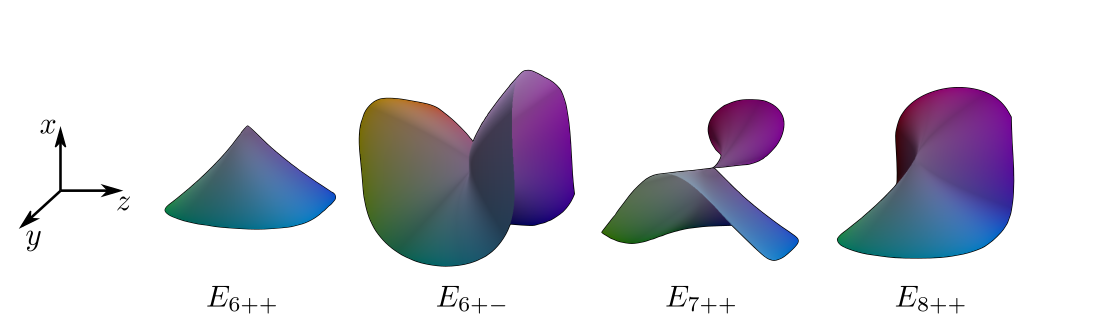
\includegraphics[scale=0.5]{images/img12}}
    \caption[$E_n$ singularities.]
    {$E_n$ singularities \cite{morris2003client}.}
    %id obrazku, pomocou ktoreho sa budeme na obrazok odvolavat
    \label{img:12}
\end{figure}
Both $E_{6++}$ and $E_{6+-}$ are topologically equivalent to a plane, thus
they each have only one branch. The planes of symmetry of both of these 
branches are $y=0$ and $z=0$, therefore we pick $(-1, 0, 0)$ as the
triangulation vector.

$E_{7++}$ singularity is topologically equivalent to a cone, therefore it has
two branches. The plane of symmetry of this singularity is $z=0$.

$E_{8++}$ singularity is also topologically equivalent to a plane, therefore
it has only one branch. This branch has only one plane of symmetry $z=0$.

We again look at the intersection of the surfaces with the plane of 
symmetry, this is displayed on the Figure \ref{img:10}.

\begin{figure}
    \centerline{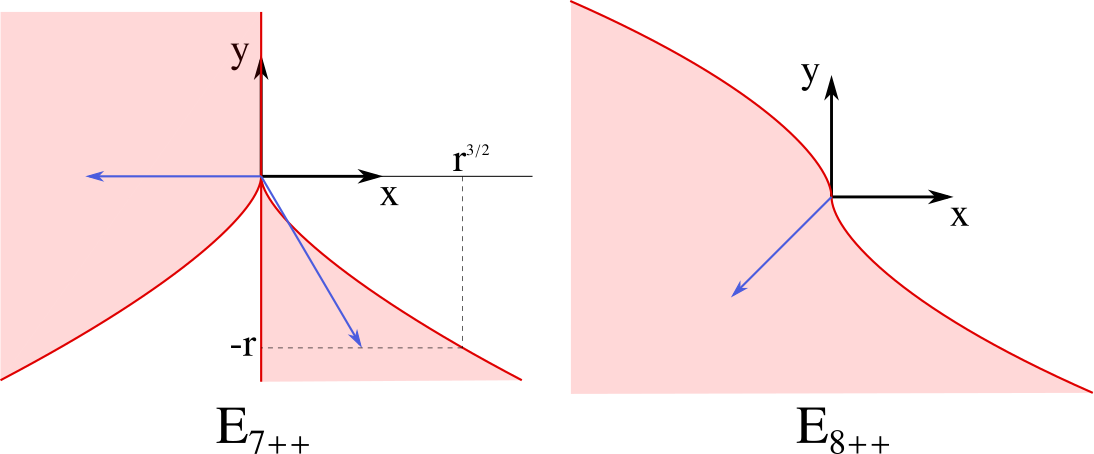
\includegraphics[scale=0.5]{images/img10}}
    \caption[Intersection of $E_{7++}$ and $E_{8++}$ singularities with 
    plane $z=0$.]
    {Intersection of $E_{7++}$ and $E_{8++}$ singularities with 
    plane $z=0$.}
    %id obrazku, pomocou ktoreho sa budeme na obrazok odvolavat
    \label{img:10}
\end{figure}

For $E_{7++}$ singularity, we pick $(-1, 0, 0)$ and 
$(\frac{1}{2}r^{\frac{3}{2}}, -r, 0)$ as triangulation vectors.
For $E_{8++}$ singularity, we pick $(-1, -1, 0)$ as a triangulation vector.
These vectors are displayed on the Figure \ref{img:10} as blue arrows.

\subsection{Analytical calculation of local triangulation of some ADE singularities}
For given edge size $e$, we calculate the local triangulation of ADE
singularities, such that edges on the border of the local triangulation
have length $e$.
\subsubsection*{$A_{n--}$ singularities}
For $A_{n--}$ singularities, we create a disc of six isosceles triangles
with vertex in the singular point. The bases of these triangles create regular
hexagon in the plane $P$ parallel to the plane $x=0$, as showed on the Figure
\ref{img:11}.
\begin{figure}
    \centerline{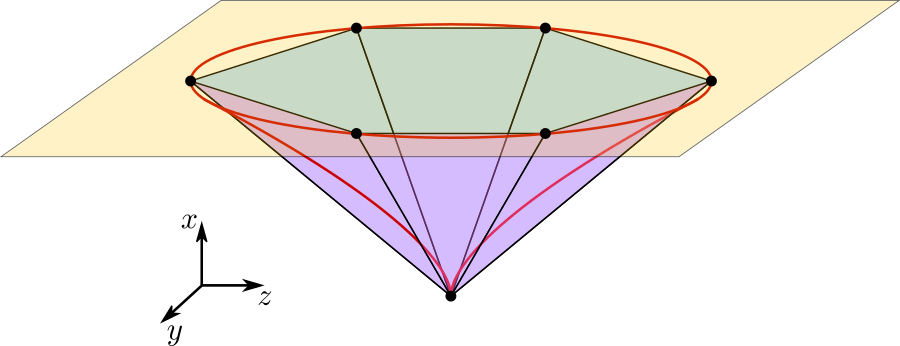
\includegraphics[scale=0.5]{images/img11}}
    \caption[Triangulation of $A_{n--}$ singularity.]
    {Triangulation of $A_{n--}$ singularity.}
    %id obrazku, pomocou ktoreho sa budeme na obrazok odvolavat
    \label{img:11}
\end{figure}
Given by equation $x^{n+1}-y^2-z^2=0$, we find the distance of the 
plane $P$ from the plane $x=0$ for the given length $e$ of the sides of
the hexagon.

Let $e$ be the length of the side of the hexagon, then the circumscribed
circle has radius $e$. This circle is identical with the intersection of
the surface and the plane $x=h$. The equation of the intersecting circle
is $y^2+z^2=h^{n+1}$ therefore, the radius can be also expressed as 
$r=h^{\frac{n+1}{2}}$, which emerges $h=e^{\frac{2}{n+1}}$. Knowing the
distance of the plane, one can easily calculate the length of the arms of
the triangles using Pythagorean theorem: 
$$a^2=h^2+e^2 \implies a = \sqrt{e^{\frac{4}{n+1}} + e^2}$$

\textbf{Layers for $A_{n--}$ singularities:}
The resulting mesh with uniform triangles for $A_{5--}$ singularity is displayed
on the Figure \ref{img:A5-uniform}.  

\begin{figure}
    \centerline{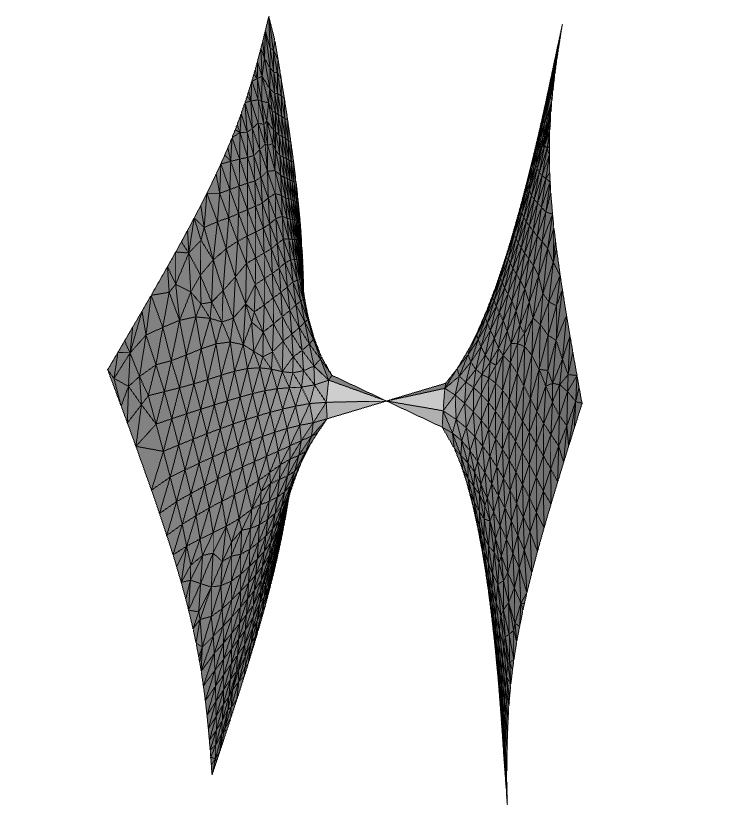
\includegraphics[scale=0.25]{images/A5-uniform}}
    \caption[Resulting uniform triangulation of the $A_{5--}$ singularity]
    {Resulting uniform triangulation of the $A_{5--}$ singularity.}
    %id obrazku, pomocou ktoreho sa budeme na obrazok odvolavat
    \label{img:A5-uniform}
\end{figure}

As one may see, the approximation around the singular
point is not as accurate as for the rest of the surface.
For this problem, we introduce layers -- the surroundings of sungularities are
triangulated in multiple layers of triangles and only after that, the algorithm for
regular parts is used.

Given the edge length $e$ and number of the layers, we calculate the height $h_e$ 
at which the bases of the triangles
have the length $e$. We divide the height by the number of layers to obtain the
layer height $h_l$. Now, $i$--th layer of points is obtained by using the height
$h = i\cdot h_l$. As we want to connect these points into triangles, every second
layer is rotated by $\frac{\pi}{6}$. The resulting 3 layers of triangles
for the $A_{1--}$ singularity as viewed from the point $(1, 0, 0)$ is displayed on
the Figure \ref{img:52}. 

\begin{figure}
    \centerline{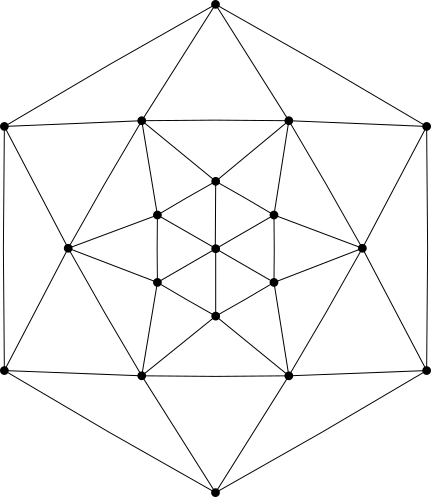
\includegraphics[scale=0.5]{images/img52}}
    \caption[Three layers of triangles for the $A_{1--}$ singularity]
    {Three layers of triangles for the $A_{1--}$ singularity.}
    %id obrazku, pomocou ktoreho sa budeme na obrazok odvolavat
    \label{img:52}
\end{figure}

The local mesh with 1 layer, 4 layers and 8 layers (from left to right) 
for $A_{5--}$ singularity is displayed
on the Figure \ref{img:53}. 
\begin{figure}
    \centerline{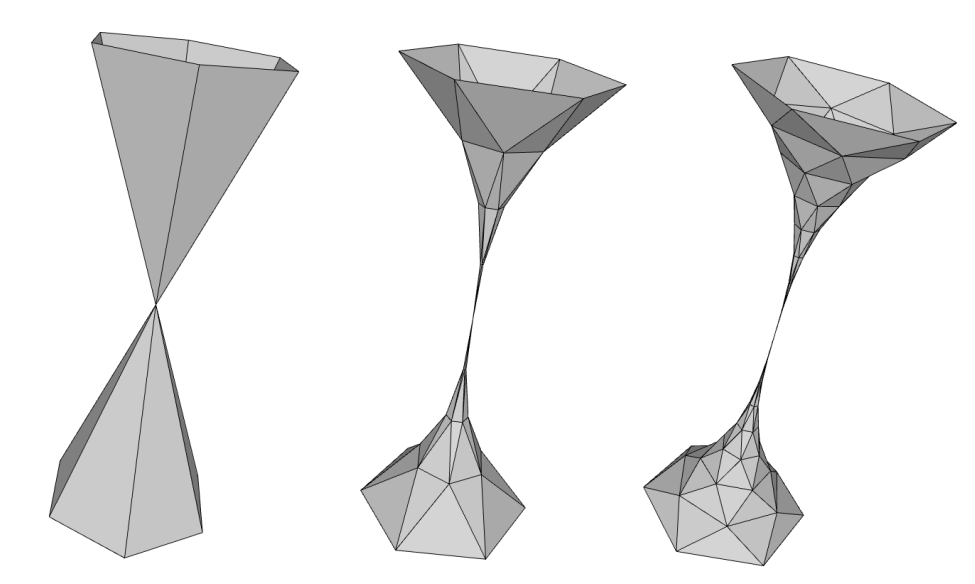
\includegraphics[scale=0.4]{images/img53}}
    \caption[Local mesh with layers for the $A_{5--}$ singularity]
    {Local mesh with 1 layer, 4 layers and 8 layers (from left to right) 
    for the $A_{5--}$ singularity.}
    %id obrazku, pomocou ktoreho sa budeme na obrazok odvolavat
    \label{img:53}
\end{figure}

The resulting mesh with 4 layers is displayed on the
Figure \ref{A5-uniform-layers}.
\begin{figure}
    \centerline{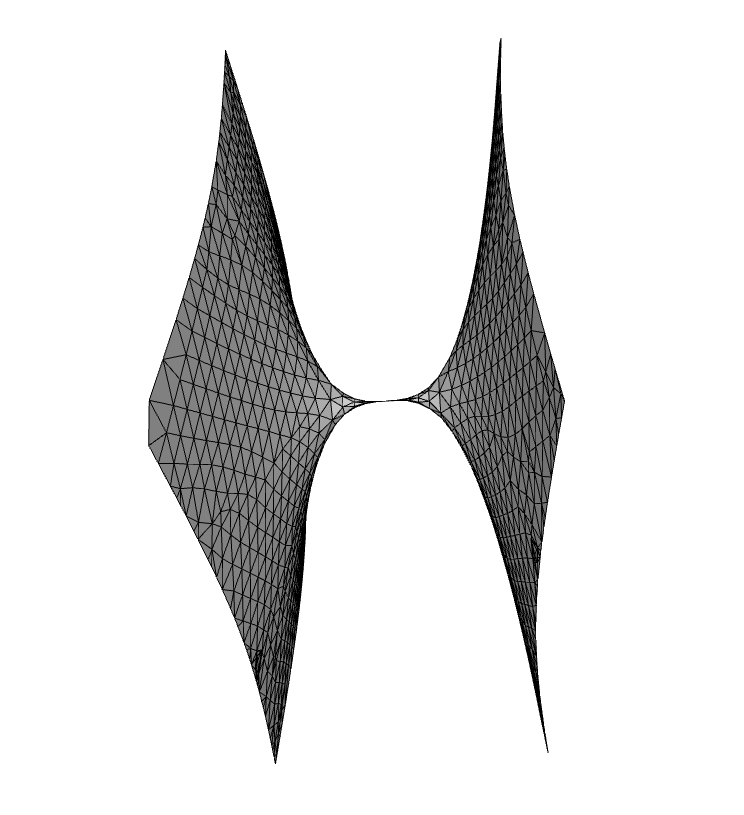
\includegraphics[scale=0.25]{images/A5-uniform-layers}}
    \caption[Resulting mesh for the $A_{5--}$ singularity]
    {Resulting mesh for the $A_{5--}$ singularity - 5 layers.}
    %id obrazku, pomocou ktoreho sa budeme na obrazok odvolavat
    \label{img:A5-uniform-layers}
\end{figure}

\subsubsection*{$D_n$ singualrities}
Some $D_n$ singularities have branches with elliptical intersection with 
a plane parallel to the plane $y=0$. As ellipses have two axes of symmetry,
we create eight triangles with apex in the singular point for these branches.
The other points of the triangles lie on the ellipse and they have the same length
of the base.

Let us have an ellipse $E$ with semi-major axis $a$, semi-minor axis $b$ 
and the center in the point $(0, 0)$.

$$E: \frac{x^2}{a^2} + \frac{y^2}{b^2} = 1$$
\begin{figure}
    \centerline{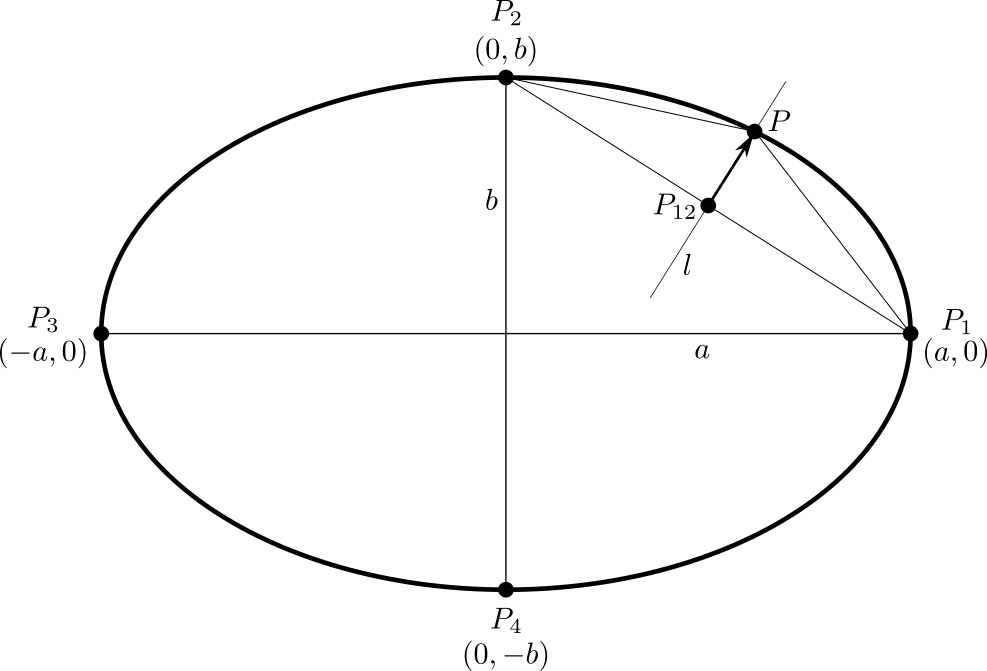
\includegraphics[scale=0.5]{images/img13}}
    \caption[Equidistant points on ellipse.]
    {Equidistant points on ellipse.}
    %id obrazku, pomocou ktoreho sa budeme na obrazok odvolavat
    \label{img:13}
\end{figure}
As displayed on the Figure \ref{img:13}, we pick the leftmost, the rightmost, the top
and the bottom points. As shown on the figure \ref{img:13}, the coordinates of these 
points are $P_1 = (a, 0)$, $P_2 = (0, b)$, $P_3=(-a, 0)$, $P_4 = (0, -b)$.
Then we can calculate the point $P$ on ellipse equidistant
from points $P_1$ and $P_2$. We calculate this point by taking the point $P_{12}$ 
in the middle of a line segment $P_1P_2$. 

$$P_{12} = \frac{1}{2}(a, b)$$

Then, the point $P$ is lying on the
intersection of the ellipse and a line $l$ passing through the point $P_{12}$, perpendicular to the
line segment $P_1P_2$.

$$l: \frac{1}{2}(a,b) + \frac{t}{2}(b,a), \hspace{3mm} t \in \R$$

Given the ellipse with semi-major axis $a$, 
semi-minor axis $b$ and the center in the point $(0, 0)$, the point $P$ can be 
calculated as follows:

$$P \in l \cap E \implies 
\frac{(a+tb)^2}{4a^2} + \frac{(b+ta)^2}{4b^2} = 1$$
$$t=\frac{ab(\sqrt{3a^4+2a^2b^2+3b^4}-a^2-b^2)}{a^4+b^4},$$

therefore 
$$P=\frac{1}{2}(a,b) + \frac{ab(\sqrt{3a^4+2a^2b^2+3b^4}-a^2-b^2)}{2(a^4+b^4)}(b,a).$$

Given edge length $e$, we are not able to calculate the height in which the distance
between points $P1$ and $P$ is $e$. The visualization showing this is on the Figure \ref{img:17}.

\begin{figure}
    \centerline{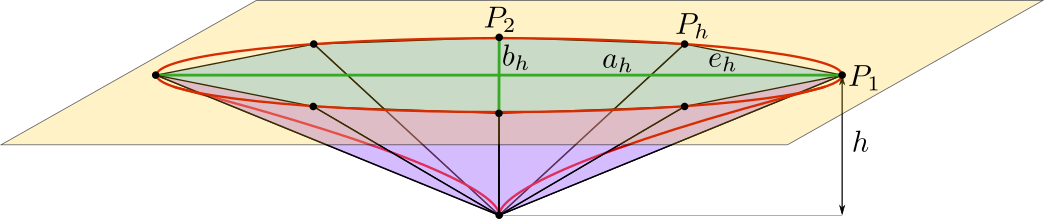
\includegraphics[scale=0.5]{images/img17}}
    \caption[Calculating the point $P_h$]
    {Calculating the point $P_h$ -- point on the ellipse equidistant from $P_1$ and $P_2$.}
    %id obrazku, pomocou ktoreho sa budeme na obrazok odvolavat
    \label{img:17}
\end{figure}

We use binary search to find such height.
Given the height and the singularity class, we can calculate the semi-major axis
and semi-minor axis as 

$$D_{n+-} \hspace{3mm} :\hspace{3mm}  -hx^2+h^{n-1}-z^2 = 0 \hspace{5mm} h>0$$
$$x^2 + \frac{z^2}{h} = h^{n-2}$$
$$\frac{x^2}{h^{n-2}} + \frac{z^2}{h^{n-1}} = 1 \implies a_h=max(h^\frac{n-2}{2}, h^\frac{n-1}{2}) \land b_h=min(h^\frac{n-2}{2}, h^\frac{n-1}{2}).$$

As we can see, we get the same ellipse for $D_{n--}$ singularities:

$$D_{n--} \hspace{3mm} :\hspace{3mm}  -hx^2-h^{n-1}-z^2 = 0 \hspace{5mm} h>0$$
$$2|n \land x^2 + \frac{z^2}{h} = -h^{n-2} \implies x^2 + \frac{z^2}{h} = h^{n-2}.$$
Then 
$$P_h=\frac{1}{2}(h^\frac{n-2}{2},h^\frac{n-1}{2}) + \frac{h^\frac{2n-3}{2}(\sqrt{3h^{2n-4}+2h^{2n-3}+3h^{2n-2}}-h^{n-2}-h^{n-1})}{2(h^{2n-4}+h^{2n-2})}(h^\frac{n-1}{2},h^\frac{n-2}{2})$$
$$P_h=\frac{1}{2}(h^\frac{n-2}{2},h^\frac{n-1}{2}) + \frac{h^\frac{1}{2}(\sqrt{3+2h+3h^2}-1-h)}{2(1+h^2)}(h^\frac{n-1}{2},h^\frac{n-2}{2})$$
and we can calculate $e_h=||P_h-P_1||$.

As $e \leq a_h$, we can start the binary search on the interval
$\langle 0, a^\frac{2}{n-2}\rangle$ or $\langle 0, a^\frac{2}{n-1}\rangle$
and finish, when required precision is reached.

\textbf{Proof that $e_h$ is monotone in $h$:} Let us consider a general ellipse
with the semi-major axis $a$, semi-minor axis $b$ and center in the point $(0, 0)$. 
Let us denote the points as follows: $A=(a, 0)$, $B=(0, b)$, $M=(\frac{a}{2}, \frac{b}{2})$ 
and $C$ - point in the first quadrant of the ellipse equidistant from $A$ and $B$, the points
are displayed on the Figure \ref{img:40}.

\begin{figure}
    \centerline{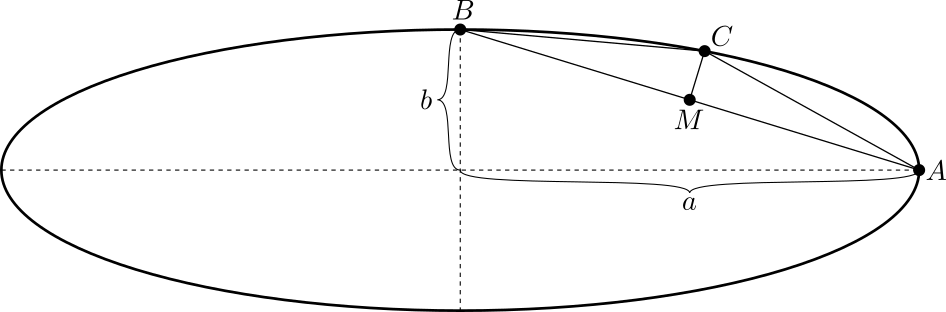
\includegraphics[scale=0.5]{images/img40}}
    \caption[Notation used in the proof]
    {Notation used in the proof that $e_h$ is monotone in $h$.}
    %id obrazku, pomocou ktoreho sa budeme na obrazok odvolavat
    \label{img:40}
\end{figure}

As we calculated, it holds, that
$$C = M + \frac{t}{2} \cdot (b, a) \hspace{5mm} \textrm{for} \hspace{5mm} t=\frac{ab(\sqrt{3a^4+2a^2b^2+3b^4}-a^2-b^2)}{a^4+b^4}.$$

As length of the vector $(b,a)$ is $\sqrt{a^2+b^2}$, the distance 
$|MC|$ is $\frac{t}{2} \cdot \sqrt{a^2+b^2}$.

After substituing for $t$, one gets 
$$|MC|=\sqrt{a^2+b^2}\cdot\frac{ab(\sqrt{3a^4+2a^2b^2+3b^4}-a^2-b^2)}{2(a^4+b^4)},$$
the derivative $\frac{\partial|MC|}{\partial a}$ is positive for all $b>0$ and
$\frac{\partial|MC|}{\partial b}$ is positive for all $a>0$.

This means that $|MC|$ is increasing in both $a$ and $b$. As the distance $|MA|=|MB|$ is 
also increasing in $a$ and $b$, it follows from Pythagorean theorem, that $|AC|=|BC|$
is increasing in $a$ and $b$.

When the height $h$ increases, both semi-major and semi-minor axis of the ellipse increase,
thus $e_h$ is increasing in $h$.

\subsection{Numerical calculation of local triangulation of ADE singularities}

For other types of ADE singularities, the exact analytical calculations become more
complicated. In this section we present an approach for triangulation of all types
of ADE singularities using iterative numerical algorithms based on the idea of binary 
search.

We begin by dividing ADE singularities into two categories.
\begin{enumerate}
    \item Category singularities -- displayed on the Figure \ref{img:42}:
    \begin{itemize}
        \item $A_{n--}$,
        \item $A_{n+-}$,
        \item $D_{n+-}$, where $n=2k$,
        \item $E_{6++}$, 
        \item $E_{6+-}$,
        \item $E_{8++}$.
    \end{itemize}
    \begin{figure}
        \centerline{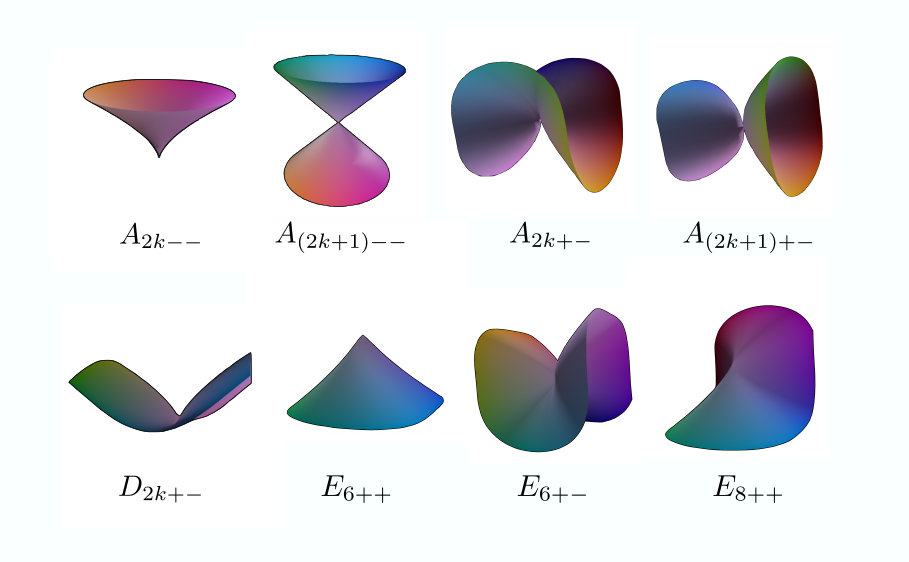
\includegraphics[scale=0.5]{images/img42}}
        \caption[1. Category singualrities]
        {1. Category singularities \cite{morris2003client}.}
        %id obrazku, pomocou ktoreho sa budeme na obrazok odvolavat
        \label{img:42}
    \end{figure}
    \item Category singularities -- displayed on the Figure \ref{img:43}:
    \begin{itemize}
        \item $D_{n+-}$, where $n=2k+1$,
        \item $D_{n--}$,,
        \item $E_{7++}$.
    \end{itemize}
    \begin{figure}
        \centerline{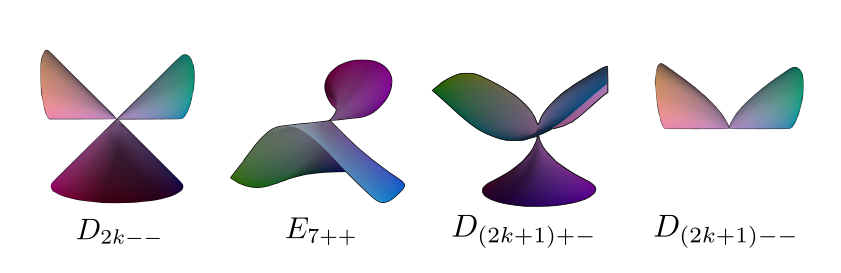
\includegraphics[scale=0.5]{images/img43}}
        \caption[2. Category singularities]
        {2. Category singularities \cite{morris2003client}.}
        %id obrazku, pomocou ktoreho sa budeme na obrazok odvolavat
        \label{img:43}
    \end{figure}
\end{enumerate}

\subsubsection*{Triangulation of 1. category singularities}
For all of the singularities, we have defined the triangulation vector,
let us denote the normalized triangulation vector for the singularity of the 
type $T$ as $\vec{t}_T$, resp. $\vec{t}_T^1, .., \vec{t}_T^i$ if the 
singularity has $i$ triangulation vectors.
Let us assume that the singular point is located in the point $O = (0, 0, 0).$
For the singularities from 1. category, 
topologically equivalent to a plane, given by the implicit
equation $F(x, y, z) = 0$ it holds, that $F(O+\vec{t}_T) \cdot F(O-\vec{t}_T)<0$.
For the singularities from 2. category, topologically equivalent to a cone,
it holds, that $F(O+\vec{t}_T) \cdot F(O+\vec{t}_T^\bot)$.
This means, that in both cases, we can perform binary search to find a point on 
the surface.
Given the required approximate length $l$, we perform binary search to find
an angle, for which the endpoint of the rotated vector $l \cdot \vec{t}_T$ lies on 
the surface with given precision as displayed on the Figure \ref{img:41}.

\begin{figure}
    \centerline{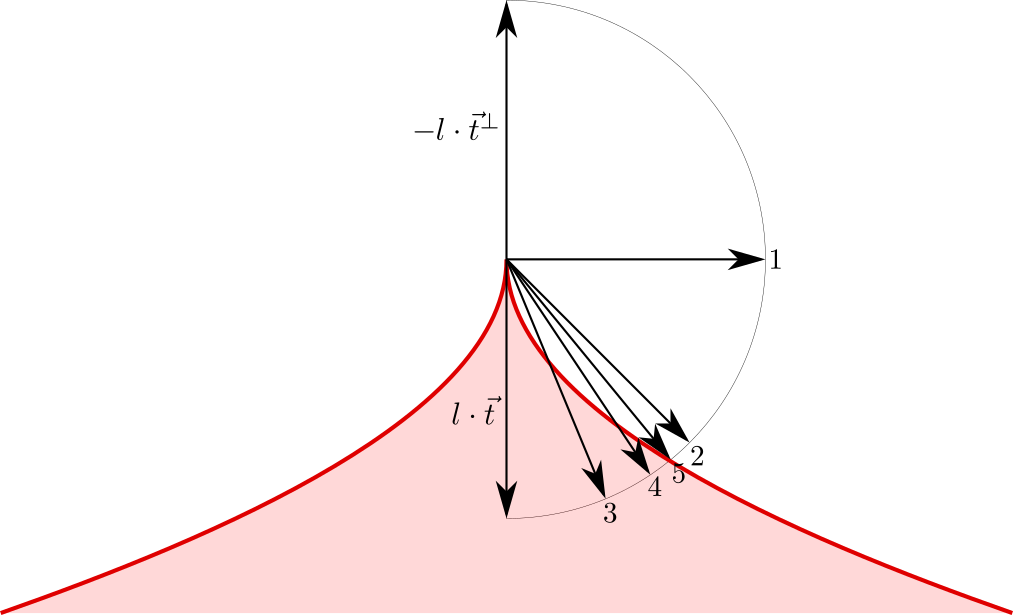
\includegraphics[scale=0.5]{images/img41}}
    \caption[Binary search for the point on the surface]
    {Binary search for the point on the surface.}
    %id obrazku, pomocou ktoreho sa budeme na obrazok odvolavat
    \label{img:41}
\end{figure}

The binary search is performed in the half-planes passing through the point
$O$ and with the vector $\vec{t}_T$ lying in the half-planes.
Using this approach, we create $k$ points on the surface, while each time
rotating the half-plane in which the binary search is performed by $\frac{2\pi}{k}$
about the axis given by $\vec{t}_T$ as displayed on the Figure \ref{img:rotating-planes}.

\begin{figure}
    \centerline{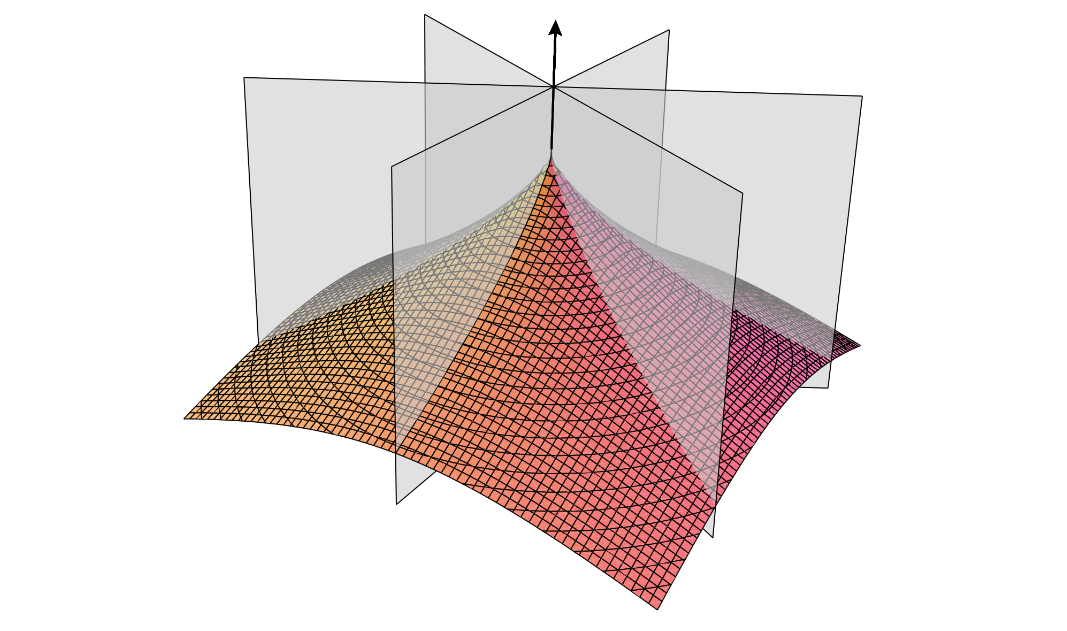
\includegraphics[scale=0.3]{images/rotating-planes}}
    \caption[Rotating the plane about the vector]
    {Rotating the plane about the vector $\vec{t}_T$.}
    %id obrazku, pomocou ktoreho sa budeme na obrazok odvolavat
    \label{img:rotating-planes}
\end{figure}

For $A_{n--}$ singularities, we create six
triangles near the singular point. We only need to perform the binary search once,
other points are obtained by rotating the point on the surface about the vector 
$\vec{t}_T$ by $\frac{2 \pi}{6}$.

In case of other singualrities, we create different number of triangles:
\begin{itemize}
    \item $A_{2k+-}$ -- 8 triangles,
    \item $A_{(2k+1)+-}$ -- 6 triangles for each branch,
    \item $D_{2k+-}$ -- 8 triangles for the branch given by the 
    triangulation vector $(0,1,0)$ and 4 triangles for the branch
    given by the triangulation vector $(0,-1,0)$,
    \item $D_{(2k+1)+-}$ -- 8 triangles,
    \item $D_{2k--}$ -- 4 triangles for each branch,
    \item $E_{6++}$ -- 6 triangles,
    \item $E_{6+-}$ -- 8 triangles,
    \item $E_{7++}$ -- 6 triangles for the branch, given by the
    triangulation vector $(-1, 0, 0)$ and 4 trianfles for the other
    branch,
    \item $E_{8++}$ -- 6 triangles.
\end{itemize}

As some singularities have symmetries, we can use these symmetries
to perform the binary search less times and find the remaining points
as the mirror symmetries of the points found by binary search.

TODO rewrite subsubsection
\subsubsection*{Triangulation of 2. category singularities}
For the singularities in the 2. category, we create more general, slower solution.
Again, we find the points on the surface, lying in the rotated half-planes
as displayed on the Figure \ref{img:rotating-planes}.
For these singularities, we do not have the general rule for the start 
and end agle to begin the binary search with. We have the triangulation vector,
whose endpoint is lying inside of the space volume bounded by the respective branch.
We consider this triangulation vector as a start vector to start the binary 
search. We find the end vector by rotating the triangulation vector $\vec{t}_T$ 
around the vector $\vec{p}_T$ -- vector perpendicular to $\vec{t}_T$, by small increments, 
until the endpoint of the vector is outside of the space volume bounded by the branch,
let us denote this vector $\vec{r}_T$.
To find the point of surface, we perform an angular binary search between $\vec{t}_T$
and $\vec{r}_T$. We proceed to find other points by rotating $\vec{p}_T$
around $\vec{t}_T$ by $\frac{2\pi}{k}$.
By using the small increments, we ensure that the rotated vector does not end up in
the space volume bounded by another branch, but it slows down the process of creating
the local mesh.
For the illustration, on the Figure \ref{img:54} on the left one can see the iterative
process to find the vector $\vec{r}_T$ by rotating $\vec{t}_T$ around $\vec{p}_T$.
On the right, one can see the rotation of $\vec{p}_T$ around $\vec{t}_T$ by 
$\frac{2pi}{k}$ to find the remainding points on the surface.


\begin{figure}
    \centerline{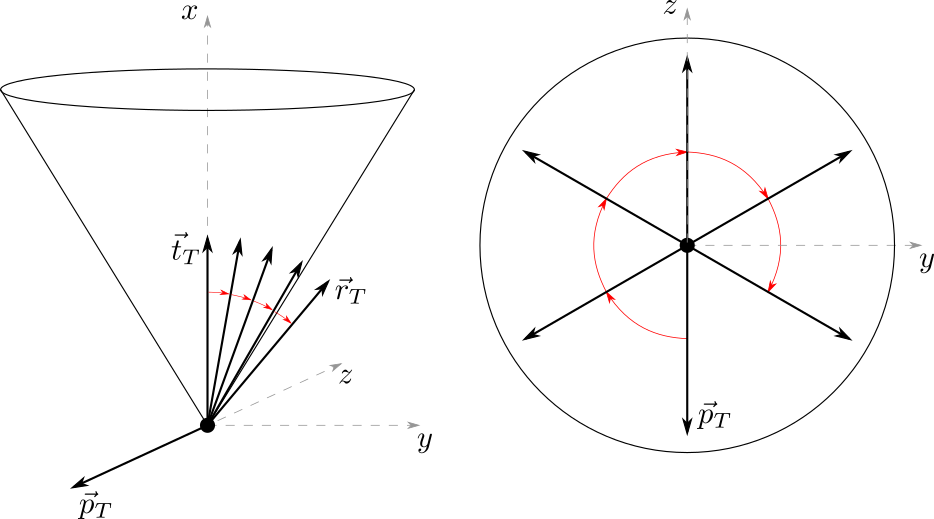
\includegraphics[scale=0.5]{images/img54}}
    \caption[TODO]
    {TODO.}
    %id obrazku, pomocou ktoreho sa budeme na obrazok odvolavat
    \label{img:54}
\end{figure}


\begin{figure}
    \centerline{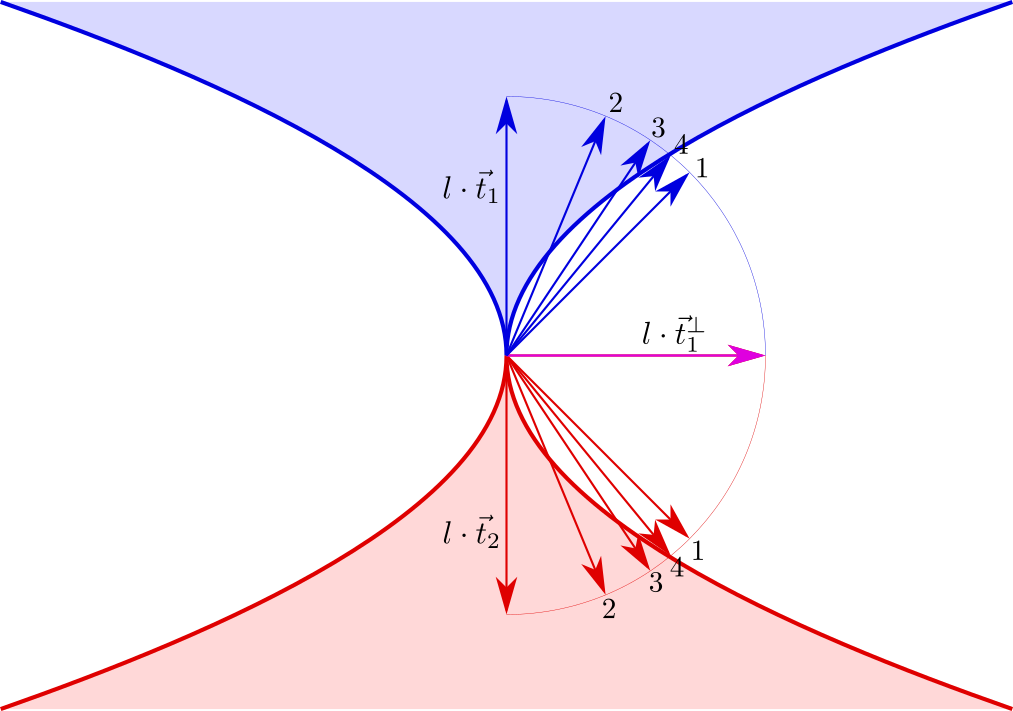
\includegraphics[scale=0.5]{images/img45}}
    \caption[Double binary search for the point on the surface]
    {Double binary search for the point on the surface.}
    %id obrazku, pomocou ktoreho sa budeme na obrazok odvolavat
    \label{img:45}
\end{figure}

For the singularities with symmetrical branches, we only need to perform binary
search in one of the half-spaces. In case of the singularities with rotation
symmetry, we again create six triangles and only need to perform the binary search once.
In case of other singularities, we create eight triangles, while again making use of the
potential planes of symmetry.

\subsubsection*{Layers}

\subsubsection*{Optimization of the quality of the local mesh for some singularities}
For some of the singularities, it is not convinient to look for the points on
the surface in the planes rotated by identical angles as seen on the Figure
\ref{img:rotating-planes}. An example of such singularities are $D_{n+-}$
singularities. The local mesh created with 8 triangles using the described 
approach is displayed on the Figure \ref{img:D4-before}. 

\begin{figure}
    \centerline{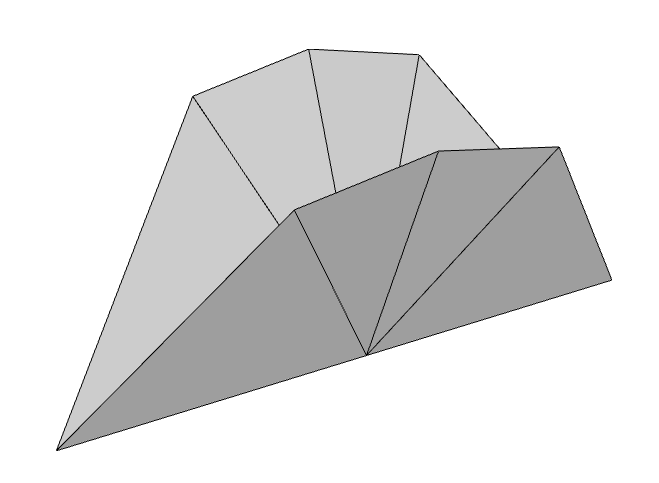
\includegraphics[scale=0.25]{images/D4-before}}
    \caption[Uneven triangles in the local mesh around $D_{4+-}$ singularity]
    {Uneven triangles in the local mesh around $D_{4+-}$ singularity.}
    %id obrazku, pomocou ktoreho sa budeme na obrazok odvolavat
    \label{img:D4-before}
\end{figure}

The problem is significant on the singularities with 8 triangles near
the singular point.
Our solution is to use binary search to find the angle where the triangles are
close to isosceles triangles. The points given by the angles 
$0, \frac{\pi}{2}, \pi$ and $\frac{3\pi}{4}$ are unchanged.
The points in between these points are iteratively changed until the
triangles are isosceles with required precision. Starting on the interval 
of angles $(0, \frac{\pi}{2})$, in each step, 
the new angle is calculated as an angle in the middle 
between the two angles, the new point is then calculated using the binary 
search to find a point on the surface as displayed on the Figure \ref{img:41}.

As all singularities using this optimization are symmetrical by two coordinate
planes, we only need to perform this binary search once for each layer of a
singularity and use mirroring to obtain the remaining points.

The result of the binary 
search of an angle on the $D_{4+-}$ singularity is displayed 
on the Figure \ref{img:D4-after}. The triangles around the singularity
are closer to isosceles triangles in comparison with the Figure 
\ref{img:D4-before}.

\begin{figure}
    \centerline{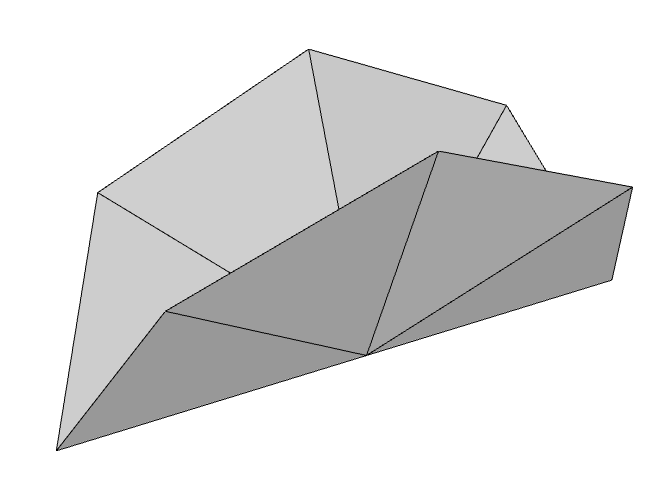
\includegraphics[scale=0.25]{images/D4-after}}
    \caption[Optimized local mesh around $D_{4+-}$ singularity]
    {Optimized local mesh around $D_{4+-}$ singularity.}
    %id obrazku, pomocou ktoreho sa budeme na obrazok odvolavat
    \label{img:D4-after}
\end{figure}

\subsection{Triangulation of a plane with multiple $A_{n--}$ singularities}
In this section, we present an approach for creating an implicit equation of a
surface which consists of a plane and arbitrary many $A_{n--}$ singularities
$C^1$ smoothly connected to this plane. 
\subsubsection*{Input and output}
In this section, the following data are provided on the input:
\begin{enumerate}
    \item the number of singularities - $m$,
    \item $m$ discrete points on a plane - $(x_1, y_1), ..., (x_m, y_m)$,
    \item $m$ degrees of the singularities - $n_1, ..., n_m$,
    \item $m$ heights at which each singularity is connected - $h_1, ..., h_m$.
\end{enumerate}
The visualisation of desired output function can be seen on the Figure \ref{img:22}. 
On this figure, the singularity is displayed by green color, the red color is used to
display the function which connects the singularity to a plane - the bump function.
\begin{figure}
    \centerline{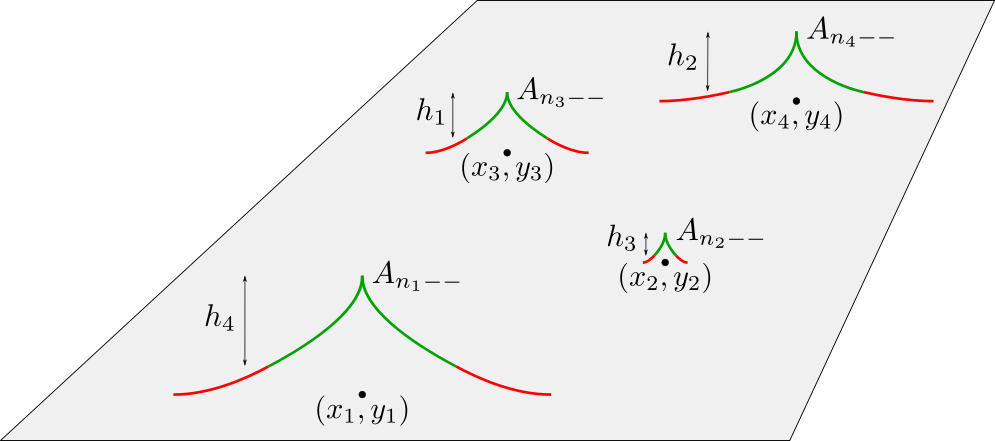
\includegraphics[scale=0.5]{images/img22}}
    \caption[Plane with singularities.]
    {Plane with singularities.}
    %id obrazku, pomocou ktoreho sa budeme na obrazok odvolavat
    \label{img:22}
\end{figure}
There are some limitations on the input data. As we do not want the singularities 
or the bump functions to intsect, we require that each pair of input points is
distanced $d_{ij}$ from each other. We specify the value of $d_{ij}$ in the section TODO.
\subsubsection*{Bump function}
\begin{definition}
The support $supp(f)$ of a function $f: \R^n \to \R$ is a set of points where $f$ is not
zero: $$supp(f) = \{ x\in \R^n : f(x)\neq 0 \}.$$
The closed support of the function $f$ is defined as a closure of $supp(f)$.
\end{definition}
Bump function if a function $f:\R^n \to \R$ which is smooth ($C^\infty$) and
compactly supported (the closed support of the function $f$ is a compact subset
of $\R^n$).

The most common example of such bump function is the function 
$$f(x)= \left\{
    \begin{array}{ll}
        e^{-\frac{1}{1-x^2}}, & x \in (-1, 1) \\
          0, & otherwise,\\
    \end{array} 
    \right. $$
which is both $C^\infty$ and compactly supported.

The bump function can be used to smoothly connect a curve to a line or a surface to a
plane in higher dimension. If we only need to connect a curve and a line $C^n$ smoothly, 
we only need a bump function which connects $C^n$ smoothly to a line.

In our work, we connect two surfaces with $C^1$ continuity and for this purpose
we use the function
$$f(x)= \left\{
    \begin{array}{ll}
        -q \cdot cos(k \cdot x)-q, & x \in (-\frac{\pi}{k}, \frac{\pi}{k}) \\
        0, & otherwise,\\
    \end{array} 
    \right. $$
rotated about $z$-axis.
The result of the rotation is the following function:
$$f(x, y) = \left\{
    \begin{array}{ll}
        -q \cdot cos(k \cdot (x^2+y^2))-q, & x^2+y^2<=(\frac{\pi}{k})^2 \\
        0, & otherwise.\\
    \end{array} 
    \right. $$
Both of these functions can be seen on the Figure \ref{img:21}.
\begin{figure}
    \centerline{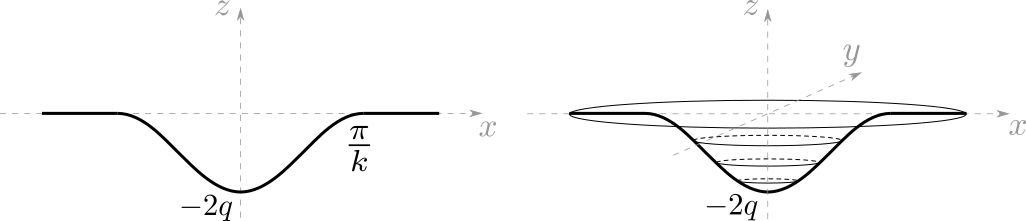
\includegraphics[scale=0.5]{images/img21}}
    \caption[$C^1$ cosine bump function.]
    {$C^1$ cosine bump function.}
    %id obrazku, pomocou ktoreho sa budeme na obrazok odvolavat
    \label{img:21}
\end{figure}

\subsubsection*{Implicit equation of the cosine bump function}
To construct the implicit equation of the cosine bump function, we use CSG
- constructive solid geometry, which is described in the section \ref{sub2.6}.

First, we cut out the part of the rotated cosine, where
$x^2+y^2<(\frac{\pi}{k})^2$ using cylinder and intersection operation. Next,
we use a plane and the union operation to \textit{glue} the bump to the plane.
The described process is displayed on the Figure \ref{img:24} in the form of CSG tree.
\begin{figure}
    \centerline{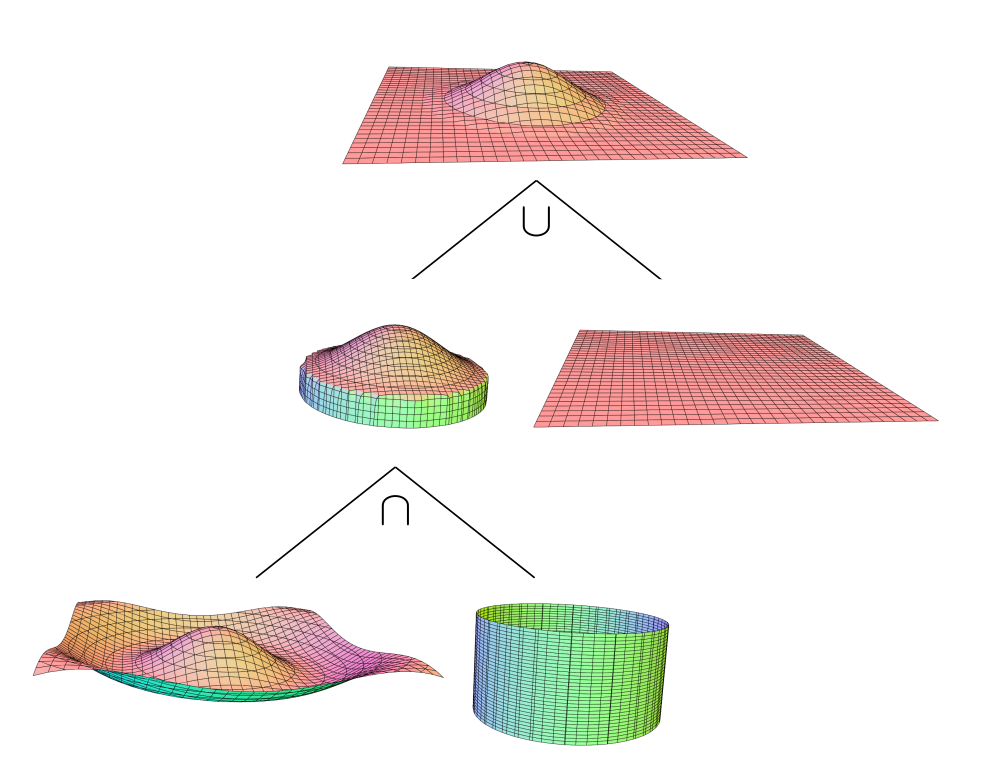
\includegraphics[scale=0.5]{images/img24}}
    \caption[Construction of the cosine bump function using CSG]
    {Construction of the cosine bump function using CSG.}
    %id obrazku, pomocou ktoreho sa budeme na obrazok odvolavat
    \label{img:24}
\end{figure}
We use the following equations of the surfaces to model the cosine bump function:

\begin{table}[]
    \centering
    \begin{tabular}{|c|c|}
        \hline\hline
    Funcion name            & Implicit equation                                        \\ \hline\hline
    Rotated cosine function & $x+q \cdot cos(k \cdot \sqrt{(y-p_y)^2+(z-p_z)^2})+q=0$  \\ \hline
    Cylinder                & $(y-p_y)^2+(z-p_z)^2-(\frac{\pi}{k})^2=0$                \\ \hline
    Plane                   & x=0                                                      \\ \hline\hline
    \end{tabular}
    \caption[Implicit equations for bump function modelling]
    {Implicit equations for bump function modelling.}
    \label{tab:1}
    \end{table}

Parameters $q$ and $k$ allow us to change the amplitude and the frequency of
the cosine function, parameters $p_y$ and $p_z$ are used to move the bump function
to the given point $(p_y, p_z)$.

\subsubsection*{Attaching singularities to the plane using the cosine bump function}

Given the type of the singularity - $n$ and given height - $h$, we calculate the
constants of the cosine bump function to connect $C^1$ smoothly to the given
singularity.

The singularity given by the implicit equation $x^{n+1}-y^2-z^2$ intersected with 
the plane $x=h$ produces a circle with the radius $r=\sqrt{h^{n+1}}$.
The cosine bump function is scaled using $q$ and $k$ to smoothly connect the
singularity in the middle of the cosine bump function. This approach is displayed
on the Figure \ref{img:25}. 

\begin{figure}
    \centerline{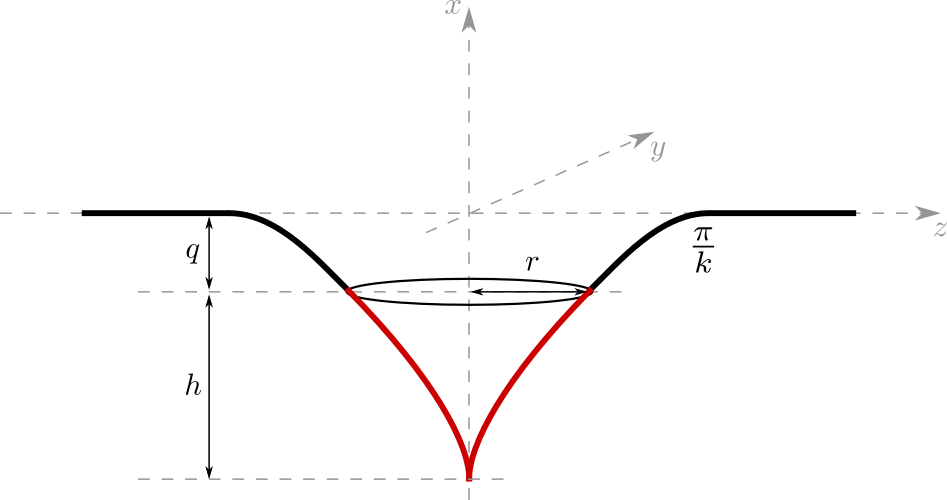
\includegraphics[scale=0.5]{images/img25}}
    \caption[Attaching the singularity to a plane using the cosine bump function]
    {Attaching the singularity to a plane using the cosine bump function.}
    %id obrazku, pomocou ktoreho sa budeme na obrazok odvolavat
    \label{img:25}
\end{figure}

As the singularity is attached in the middle of the
bump function, we get the equality $r=\frac{\pi}{2k}$ and therefore
$\sqrt{h^{n+1}}=\frac{\pi}{2k} \implies k=\pi/(2\sqrt{h^{n+1}})$.
The parameter $q$ is calculated from $C^1$ continuity requirement. We require the
gradients to be linearly dependent in the points of connection. Due to the rotation
symmetry, we check it only for the intersection with the plane $z=0$
for the point $(-q, \frac{\pi}{2k})$.
$$F=(x+h+q)^{n+1}-y^2 \implies \nabla F = \left[(n+1)(x+h+q)^n, -2y\right]$$
$$\nabla F \left(-q, \frac{\pi}{2k}\right) = \left[(n+1) h^n, -\frac{\pi}{k}\right]$$
$$G=x+q \cdot cos(k y)+q \implies \nabla G = \left[1, -qk \cdot sin(k y)\right]$$
$$\nabla G \left(-q, \frac{\pi}{2k}\right) = \left[1, -qk \right]$$

Requiring $\nabla F (-q, \frac{\pi}{2k}) = s \cdot \nabla G (-q, \frac{\pi}{2k})$
and knowing $k=\pi/(2\sqrt{h^{n+1}})$, we get $s=(n+1)h^n$ and therefore $q=4h/(\pi(n+1))$.

After calculating the parameters $q$ and $k$ of the cosine bump function, 
we proceed to connect the singularity to the bump function.
We use intersection with the plane $x=-q$ to get the sections of the singularity
and the section of the bump function and lastly, we use union of these two 
surfaces. The described process is displayed on the Figure \ref{img:26}.
Curious reader can find the detailed calculation of the implicit equation in
the appendix \ref{appA}.

\begin{figure}
    \centerline{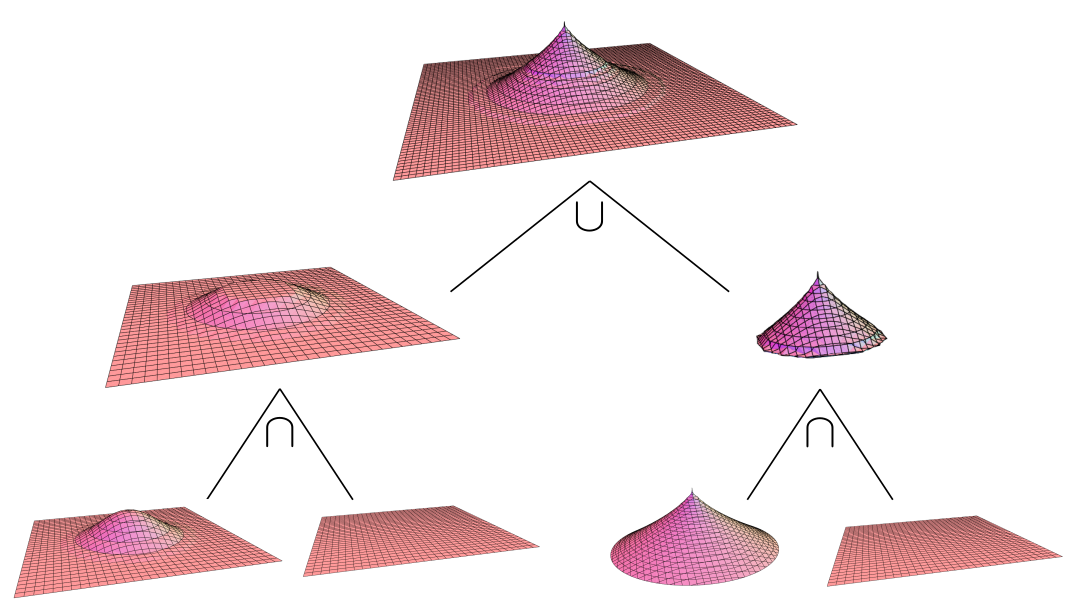
\includegraphics[scale=0.5]{images/img26}}
    \caption[Attaching the singularity to a plane using CSG]
    {Attaching the singularity to a plane using CSG.}
    %id obrazku, pomocou ktoreho sa budeme na obrazok odvolavat
    \label{img:26}
\end{figure}

To connect multiple singularities to the same plane, we construct the implicit
equation for each of these singularities and then use the union operation to
create a surface with multiple singularities. This procedure is displayed on
the Figure \ref{img:28}.

\begin{figure}
    \centerline{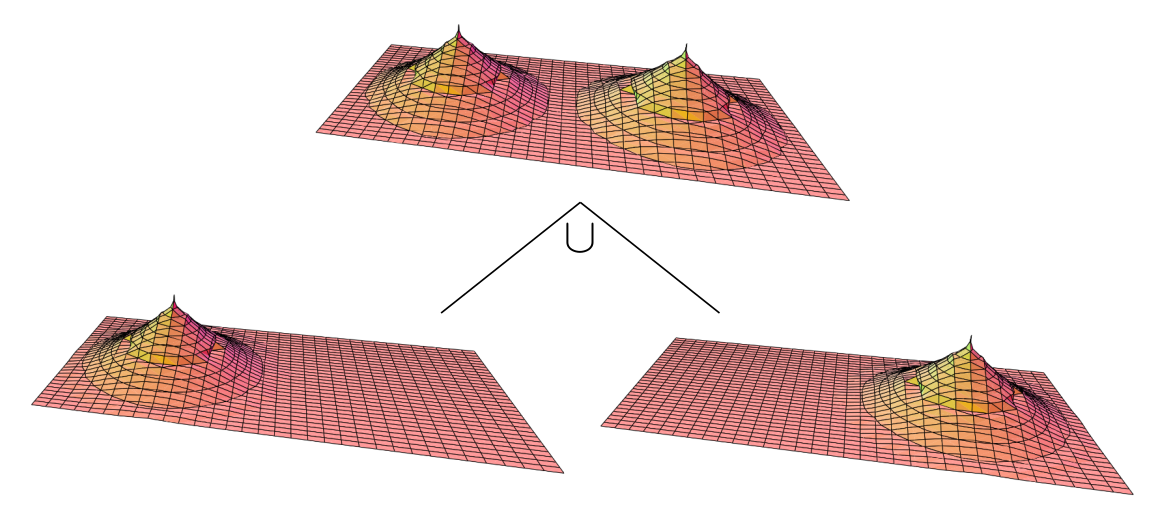
\includegraphics[scale=0.5]{images/img28}}
    \caption[Plane with multiple attached singularities]
    {Plane with multiple attached singularities.}
    %id obrazku, pomocou ktoreho sa budeme na obrazok odvolavat
    \label{img:28}
\end{figure}

\subsubsection*{Limitations on the input data}
As we already mentioned, we require that each pair of input points is
distanced $d_{ij}$ from each other. As the radius of the closed support
of the cosine bump function is $r=\frac{\pi}{k}=2\sqrt{h^{n+1}}$, the 
distance between two input points $p_j, p_j$ must be at least
$d_{ij} = 2\sqrt{h_i^{n_i+1}}+2\sqrt{h_j^{n_j+1}}$. This way, both singularities
and the corresponding bump functions do not intersect. 

\subsubsection*{Visualization of results of the triangulated surfaces}

\section{Triangulation of non-isolated singularities}
\label{sub3.3}

We present an approach for triangulation of implicit surfaces with singular
curves which are
a result of performing intersection operation on the interiors of two
regular implicit surfaces.

We start by creating a local mesh for the surroundings of these singular
curves and finish the mesh in the regular parts.

\subsection{Creating the local mesh around the singular curves}

We start by approximating the singular curve by a polyline.
On the input, one point close to the singular curve is given. This point serves as
a starting point $P_0$. The tangent vector $\vec{t}_C(P_0)$ of the curve is computed as
the cross product of the unit normal vectors of the two surfaces $S_1$ and $S_2$ given
by the implicit equations $F_1=0$ and $F_2=0$, respectively.
Given the required approximate edge length $e$, a point $Q_1$ is computed as
$Q_1 = P_0 + e \cdot \vec{t}_C(P_0)$. We obtain the point $P_1$ by projecting the point 
$Q_1$ to the curve $C$ using an approach described in the section \ref{sub2.3}.
Other points are then created iteratively by the same approach:
$$Q_{n+1} = P_n + e \cdot \vec{t}_C(P_n),$$
$$P_{n+1} = proj_C(Q_{n+1}),$$
while checking if the new point is inside the axis-aligned bounding box.
We stop once the new point is outside of the axis-aligned bounding box or
if the new point is close to the starting point $P_0$, which means the approximated
curve is a closed curve.

In case of the open curve, to complete the whole polyline, we also approximate 
the second part of the singular curve by iteratively creating points in the 
opposite direction, starting from point $P_0$. Let $m$ be number of points
in the polyline, the second part of the polyline consists of the points
$P_m, P_{m+1}, ...$, where
$$Q_m = P_0 - e \cdot \vec{t}_C(P_0),$$
$$P_m = proj_C(Q_m),$$
and again, iteratively
$$Q_{n+1} = P_n - e \cdot \vec{t}_C(P_{n}), \hspace{5mm} n = m, m+1, ...$$
$$P_{n+1} = proj_C(Q_{n+1}), \hspace{5mm} n = m, m+1, ...$$

The presented approach is visualized in two dimensions on the Figure \ref{img:37}.

\begin{figure}
    \centerline{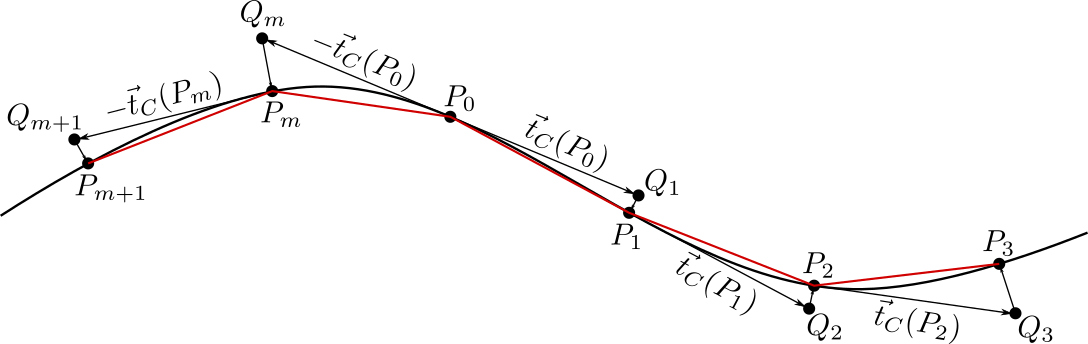
\includegraphics[scale=0.5]{images/img37}}
    \caption[Approximation of the implicit curve by polyline]
    {Approximation of the implicit curve by polyline.}
    %id obrazku, pomocou ktoreho sa budeme na obrazok odvolavat
    \label{img:37}
\end{figure}

After obtaining the polyline approximation of the curve on the intersection
of the two surfaces, one may create the local mesh. Let us rename the polyline 
points to $P_0, P_1, ..., P_k$, such that $l_i = \overline{P_i P_{i+1}}$ is a 
line segment of the polyline for $i=0, ..., k-1$ (and $l_k = \overline{P_k P_0}$ is a 
line segment of the polyline for closed curve).

For each line segment $l_i$ we create two adjacent triangles containing $l_i$.

We start by calculating the midpoint $M_i = \frac{P_i+P_{i+1}}{2}$.
By projecting the point $M_i$ to the surface $S_1$, we obtain the point $M_i^1$,
by projecting it to the surface $S_2$, we obtain the point $M_i^2$. The defiined points
are visualized on the Figure \ref{img:38}.

\begin{figure}
    \centerline{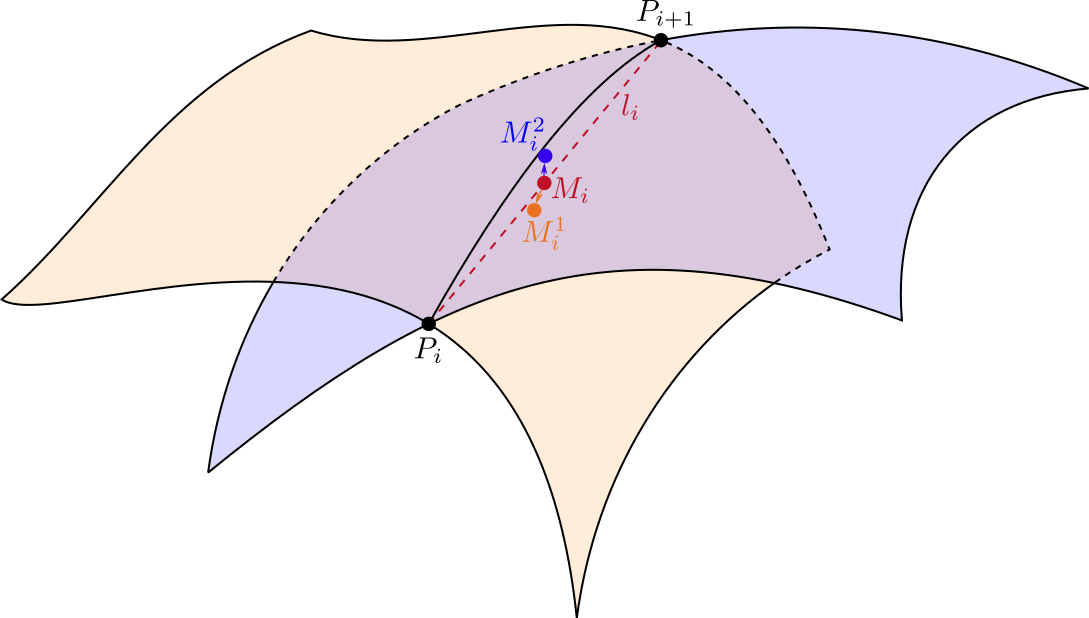
\includegraphics[scale=0.5]{images/img38}}
    \caption[Definition of the points]
    {Definition of the points $M_i$, $M_i^1$ and $M_i^2$.}
    %id obrazku, pomocou ktoreho sa budeme na obrazok odvolavat
    \label{img:38}
\end{figure}

As the point $M_i^1$ is lying on the surface, the tangent plane $T_{S_1}(M_i^1)$ 
of the surface $S_1$ in the point $M_i^1$ is well defined. The same holds for the 
point $M_i^2$ lying on the surface $S_2$. 

We first define points $R_i^1$ and $R_i^2$ close to the surface. After projecting
these points on the surface, we obtain the third point for each of the two 
adjacent triangles.

The point $R_i^1$ is obtained by moving from the point $M_i$ in the direction 
perpendicular to both $\overrightarrow{P_{i} P_{i+1}}$ and 
$\nabla{F_1}(M_1)$ by the given edge length $e$.

$$R_i^1 = M_i + e \cdot \frac{\nabla{F_1}(M_1) \times \overrightarrow{P_{i} P_{i+1}}}{||\nabla{F_1}(M_1) \times \overrightarrow{P_i P_{i+1}}||}.$$

The described situation is displayed on the Figure \ref{img:39}.
For the point $M_i$, the plane $H_i$ passing through $M_i$, perpendicular to the
line segment $l_i$ is defined:
$$H_i : \overrightarrow{P_i P_{i+1}} \cdot (X-M_i) = 0.$$
For better understanding the Figure \ref{img:39} is the projection of the surroundings
of the point $M_i$ to the plane $H_i$. Generally, points $M_i^1$ and $M_i^2$ do not lie in
the plane $H_i$. 

\begin{figure}
    \centerline{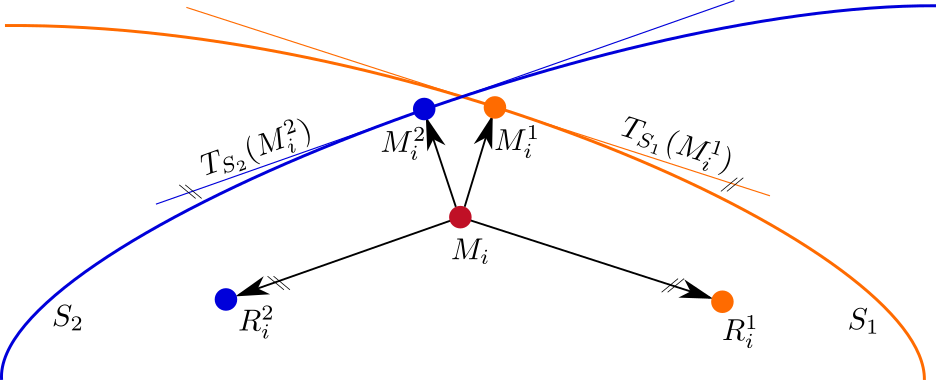
\includegraphics[scale=0.5]{images/img39}}
    \caption[Definition of the points]
    {Definition of the points $R_i^1$ and $R_i^2$ in the plane $H_i$.}
    %id obrazku, pomocou ktoreho sa budeme na obrazok odvolavat
    \label{img:39}
\end{figure}

The points $R_i^1$ and $R_i^2$ are projected to the surface given by the intersection
of the interiors of the two surfaces. The equation defining the surface is 
$$F_{1 \cap 2} = F_1 + F_2 + \sqrt{F_1^2+F_2^2}.$$

An example of the resulting local mesh for an open curve is displayed on the image
\ref{img:local-mesh-sing-curve}. This curve is a part of the singular curve on the surface 
given by the intersection of the interiors of a sphere and a hyperboloid.

\begin{figure}
    \centerline{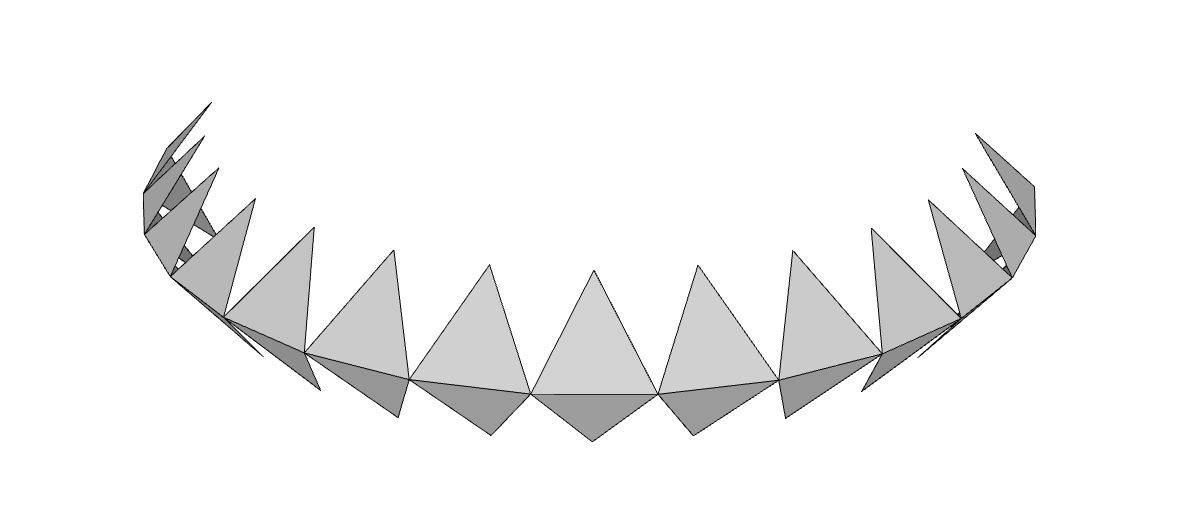
\includegraphics[scale=0.3]{images/local-mesh-sing-curve}}
    \caption[Local mesh around the singular curve]
    {Local mesh around the singular curve.}
    %id obrazku, pomocou ktoreho sa budeme na obrazok odvolavat
    \label{img:local-mesh-sing-curve}
\end{figure}